\chapter{序論}
\label{chap:introduction}

本章では,本研究の背景と本論文の構成について述べる.

\newpage

\section{背景}

Webブラウザ上での情報検索は近年広く利用されている.我々が普段情報検索を行う際,古い情報よりも新しい情報を求めていることが多い.つまり,古い情報と新しい情報を見分ける必要がある.

しかし,Web 検索の結果一覧画面における各情報は,情報の作成日時の記述はあっても,実世界に存在する紙やインクのように時間経過による外見的な劣化がないため,情報の鮮度を直感的に判断するのは難しい.

\begin{figure}[htbp]
  \begin{minipage}{0.5\hsize}
    \begin{center}
      \fbox{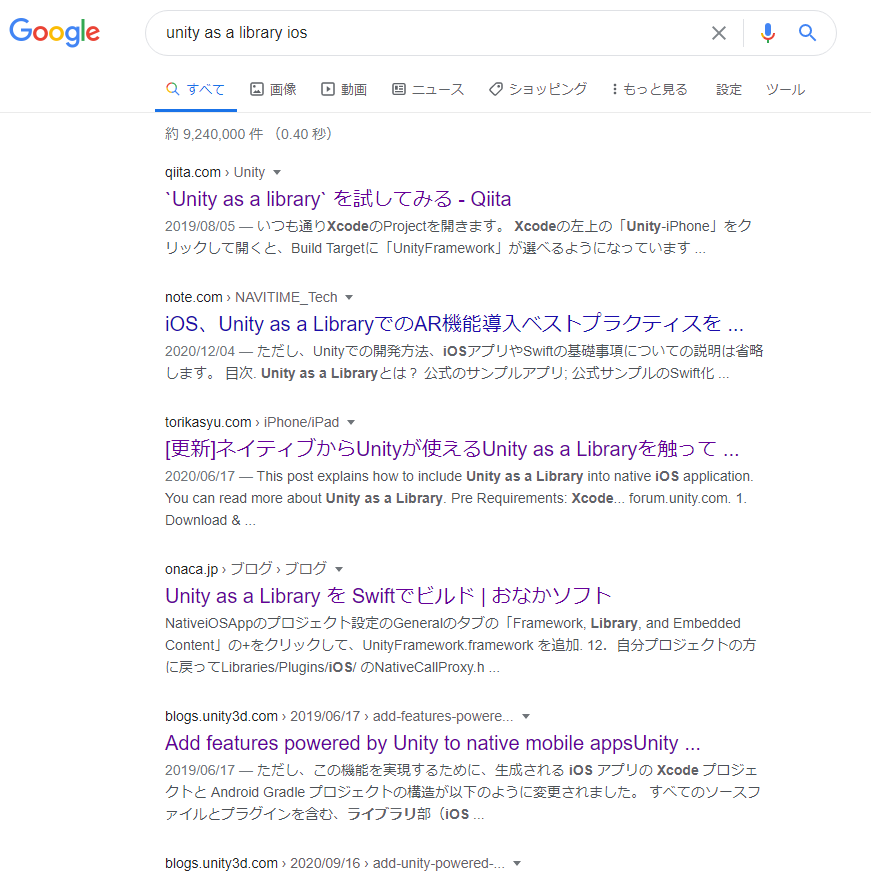
\includegraphics[width=60mm]{images/search-google.png}}
    \end{center}
    \caption{Google の検索結果一覧画面}
  \end{minipage}
  \begin{minipage}{0.5\hsize}
    \begin{center}
      \fbox{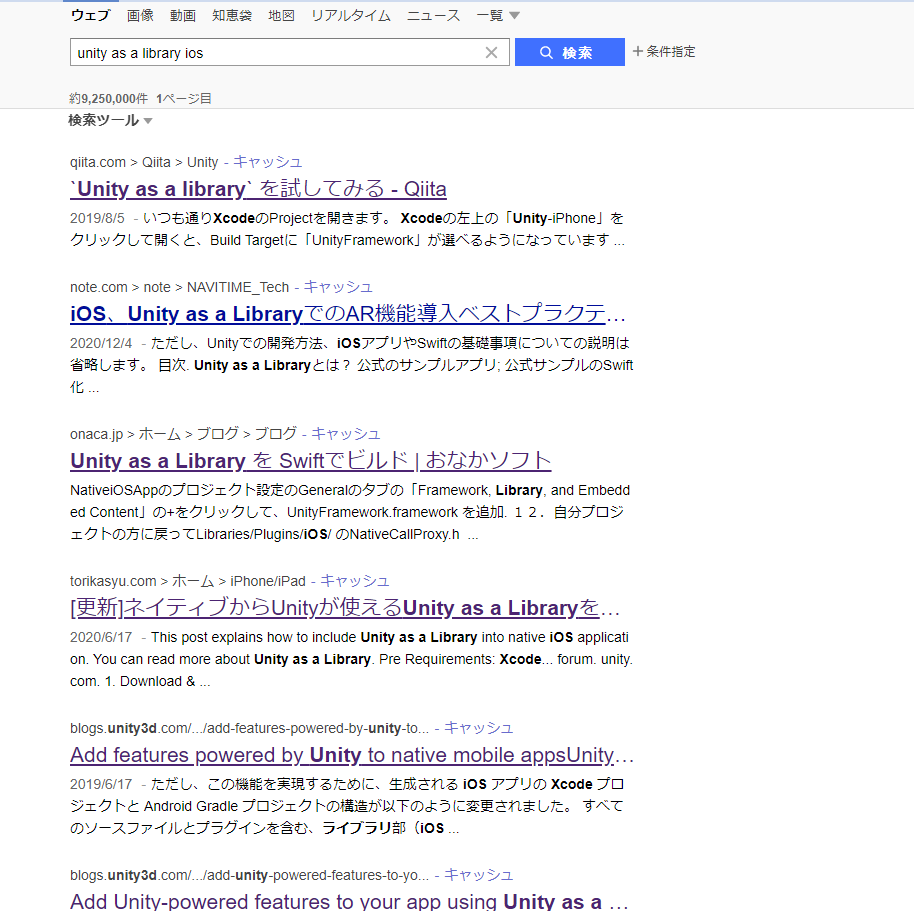
\includegraphics[width=60mm]{images/search-yahoo.png}}
    \end{center}
    \caption{Yahoo! の検索結果一覧画面}
  \end{minipage}
\end{figure}
\begin{figure}[htbp]
  \begin{minipage}{0.5\hsize}
    \begin{center}
      \fbox{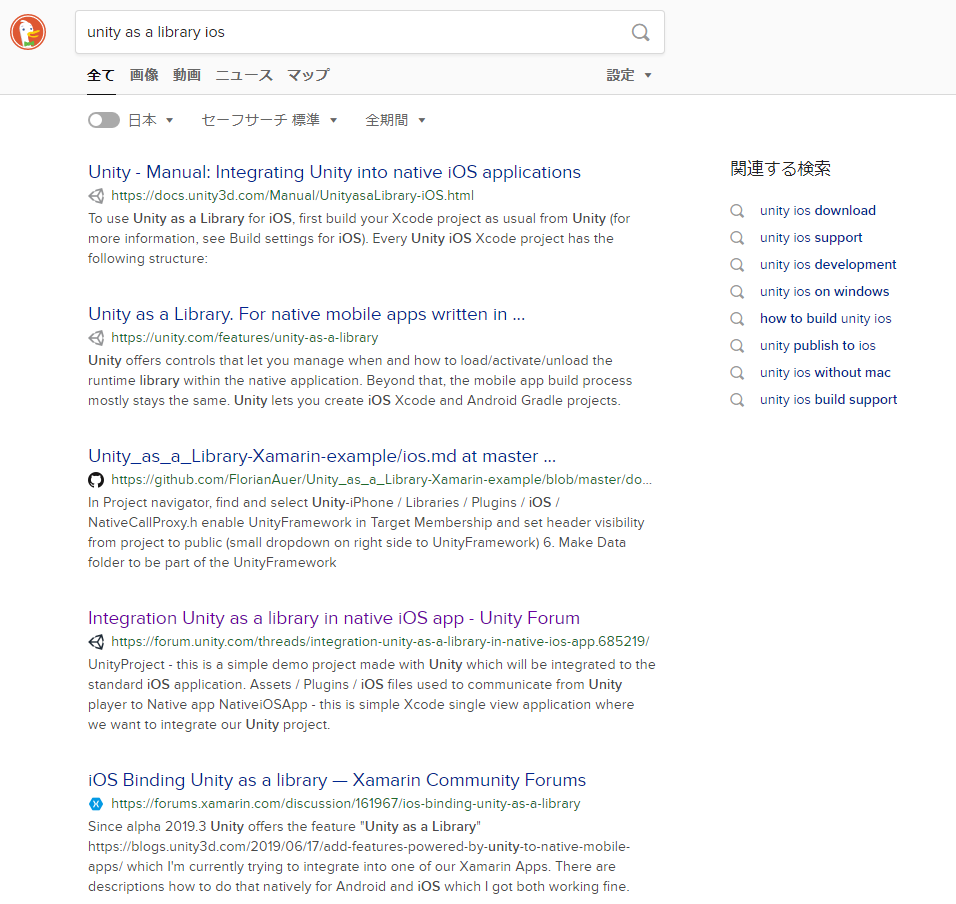
\includegraphics[width=60mm]{images/search-ddg.png}}
    \end{center}
    \caption{DuckDuckGo の検索結果一覧画面}
  \end{minipage}
  \begin{minipage}{0.5\hsize}
    \begin{center}
      \fbox{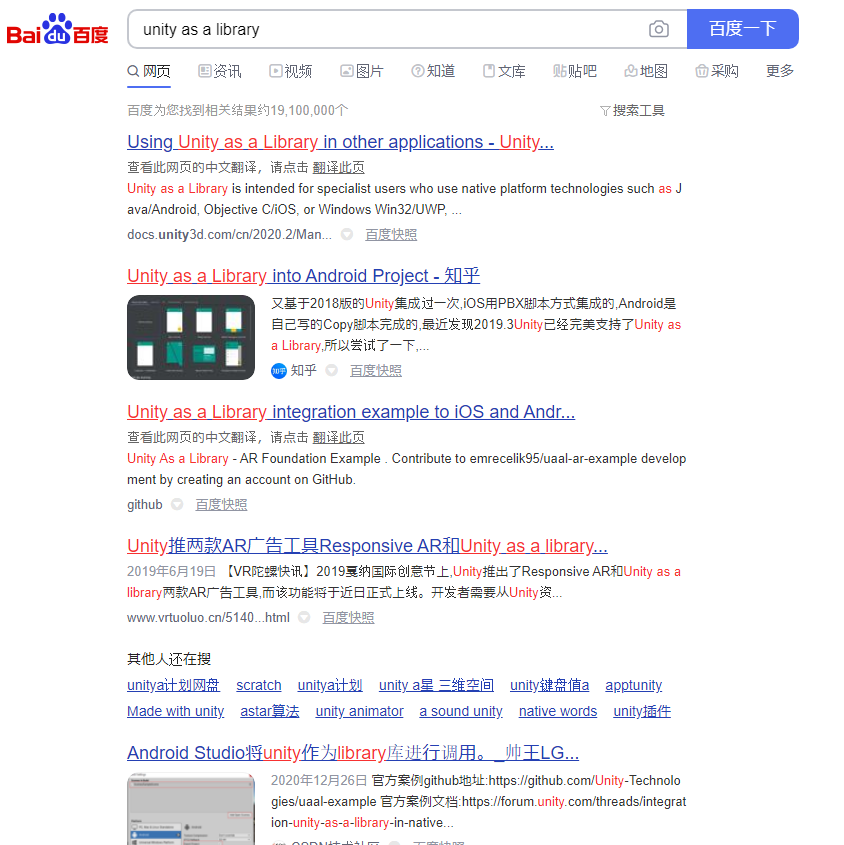
\includegraphics[width=60mm]{images/search-baidu.png}}
    \end{center}
    \caption{Baidu の検索結果一覧画面}
  \end{minipage}
\end{figure}

そこで,本来外見的な劣化のない検索結果の情報に,時間経過による表示の変化を与えることで,情報の鮮度を直感的に認識できるようになり,Web 検索による情報収集を効率的に行えると考えた.

% こういった Web 検索結果一覧画面での情報の視覚化に関して,松下らは「ネット上の情報を可視化する技術」\cite{tecvisinfo}で,

% \begin{quote}
%   Web の規模が膨大になるにつれ,ランキングの精度がますます大きな問題となるが,精度向上にも限界があるため,情報可視化システムにかかる期待も今後大きくなると予想される.
% \end{quote}

% と述べている.

% また,ユーザが検索結果から最初の選択をするまでにかける時間が平均5.7秒だという調査\cite{pinball}があり,この短い時間でユーザに情報の鮮度を認識させなければならない.
情報の鮮度を視覚化するシステムとして,リンク先のページの鮮度に応じて Web ページ内のリンクの表現を変化させる「廃れるリンク」\cite{dyinglink}のようなシステムも存在する.

しかし,検索結果一覧ページでは各リンクはリスト表示されており,それぞれに十分なスペースがあるため,より適切な鮮度の表現方法があると考えた.

\section{本研究の目的}

本研究の目的は,ユーザがより直感的に情報の鮮度を認識できるように,ブラウザにおける検索結果一覧画面の表示を拡張することである.

\section{本文書の構成}

第\ref{chap:introduction}章では本研究における背景と目的について述べる.

第\ref{chap:verification}章では実際に視覚化システムを開発する前に様々な視覚化の方法を試し評価する.

第\ref{chap:implementation}章で開発したシステムの実装に関して述べ,第\ref{chap:discussion}章では実際に利用して得られた評価や今後の展望について述べる.

第\ref{chap:survey}章では本研究と関連のある研究事例を紹介している.

第\ref{chap:conclusion}章では本研究を総括して結論を述べる.
